\documentclass{article}


\usepackage{amsmath}
\usepackage{amssymb}
\usepackage{amsfonts}
\usepackage{geometry}
\usepackage{setspace}
\usepackage{graphicx}
\usepackage{tikz}
\usepackage{xcolor}
\usepackage{multicol}
\usepackage{enumitem}
\usepackage{fancyhdr}
\usepackage{pgfplots}
\usepackage{array}
\usepackage{booktabs}
\usepackage{tabularx}
\usepackage{multirow}
\pgfplotsset{compat=1.18}
\usepackage[english]{babel}

\geometry{margin=1in}

\begin{document}

\begin{center}
    \Huge \textbf{ History Worksheet } \\[0.5cm]
    \large \textit{Generated Worksheet}
\end{center}

\vspace{1cm}

\noindent \textbf{Name:} \underline{\hspace{6cm}} \hfill \textbf{Date:} \underline{\hspace{4cm}}

\vspace{1cm}

Answer the following questions carefully.

\vspace{0.5cm}

\begin{enumerate}
\item Compare and contrast the main ideas of the Declaration of Independence with those in the Bill of Rights. \vspace{2cm} \item Analyze the historical significance of the first ten amendments to the US Constitution, known as the Bill of Rights. \vspace{2cm} \item How do the rights guaranteed by the First Amendment reflect the values of religious freedom and free speech? \vspace{2cm} \item What is the main difference between the Second Amendment's protection of the right to bear arms and the later gun control laws passed in the 20th century? \vspace{2cm} \item Sketch a graph showing the number of states that ratified the Bill of Rights over time. \vspace{2cm} \item 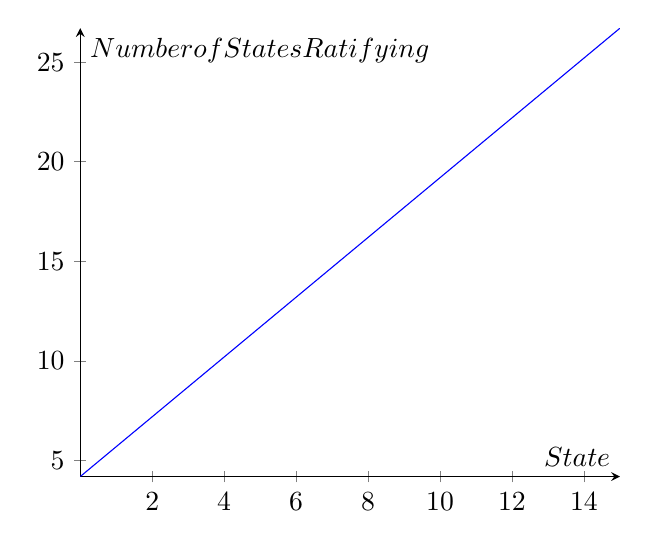
\begin{tikzpicture} \begin{axis}[ axis lines = center, xlabel = $ State $, ylabel = $ Number of States Ratifying $, ] \addplot [ domain=0:15, samples=10, color=blue, ] {4.2+1.5*x}; \end{axis} \end{tikzpicture} \vspace{2cm} \item How did the Bill of Rights influence the development of other human rights documents, such as the Universal Declaration of Human Rights? \vspace{2cm} \item Identify and explain the five freedoms protected by the First Amendment. \vspace{2cm} \item What is the significance of James Madison's role in drafting the Bill of Rights? \vspace{2cm} \item Compare and contrast the original intent behind the Second Amendment with modern-day gun control debates. \vspace{2cm} \item \begin{tikzpicture} \begin{axis}[ axis lines = center, xlabel = $ Year $, ylabel = $ Gun Violence Rate $, ] \addplot [ domain=0:10, samples=5, color=red, ] {-2.1+0.3*x}; \end{axis} \end{tikzpicture} \vspace{2cm} \item How did the Bill of Rights reflect the principles of federalism and the balance of power between the federal government and states? \vspace{2cm} \item Analyze the historical context in which the Bill of Rights was written, including the concerns about a strong central government. \vspace{2cm} \item What is the significance of the Ninth Amendment's protection of unenumerated rights? \vspace{2cm} \item \begin{tikzpicture} \begin{axis}[ axis lines = center, xlabel = $ Year $, ylabel = $ Unemployment Rate $, ] \addplot [ domain=0:10, samples=5, color=green, ] {-4.2+0.8*x}; \end{axis} \end{tikzpicture} \vspace{2cm} \item Compare and contrast the Bill of Rights with other important documents in American history, such as the Constitution and the Emancipation Proclamation. \vspace{2cm} \item How did the Bill of Rights influence the development of individual rights and liberties in the 20th century? \vspace{2cm} \item Identify and explain the three branches of government that are protected by the Bill of Rights. \vspace{2cm} \item What is the significance of the Tenth Amendment's reservation of powers to the states? \vspace{2cm} \item \begin{tikzpicture} \begin{axis}[ axis lines = center, xlabel = $ Year $, ylabel = $ GDP Growth Rate $, ] \addplot [ domain=0:10, samples=5, color=orange, ] {-2.3+1.4*x}; \end{axis} \end{tikzpicture} \vspace{2cm} \item Analyze the historical significance of the Bill of Rights in shaping American democracy and society. \vspace{2cm} \item How do the rights guaranteed by the Bill of Rights relate to modern-day social and political issues? \vspace{2cm} \item What is the main difference between the Fifth Amendment's protection of due process and the Sixth Amendment's right to a speedy trial? \vspace{2cm} \item \begin{tikzpicture} \begin{axis}[ axis lines = center, xlabel = $ Year $, ylabel = $ Poverty Rate $, ] \addplot [ domain=0:10, samples=5, color=purple, ] {-3.8+1.2*x}; \end{axis} \end{tikzpicture} \vspace{2cm} \item Compare and contrast the original intent behind the Bill of Rights with modern-day interpretations. \vspace{2cm} \item Identify and explain the three main types of amendments in the Bill of Rights: negative, affirmative, and procedural. \vspace{2cm} \item What is the significance of the Fourteenth Amendment's Due Process Clause in relation to the Bill of Rights? \vspace{2cm} \item \begin{tikzpicture} \begin{axis}[ axis lines = center, xlabel = $ Year $, ylabel = $ Education Spending Rate $, ] \addplot [ domain=0:10, samples=5, color=brown, ] {-2.1+0.9*x}; \end{axis} \end{tikzpicture} \vspace{2cm} \item Analyze the historical significance of the Bill of Rights in shaping American foreign policy and international relations. \vspace{2cm} \item How do the rights guaranteed by the Bill of Rights relate to modern-day global issues, such as human trafficking and climate change? \vspace{2cm} \item What is the main difference between the Eighth Amendment's protection against cruel and unusual punishment and the Fourteenth Amendment's Due Process Clause? \vspace{2cm} \item \begin{tikzpicture} \begin{axis}[ axis lines = center, xlabel = $ Year $, ylabel = $ Crime Rate $, ] \addplot [ domain=0:10, samples=5, color=gray, ] {-3.5+1.6*x}; \end{axis} \end{tikzpicture} \vspace{2cm} \item Compare and contrast the Bill of Rights with other important human rights documents from around the world. \vspace{2cm} \item Identify and explain the three main principles of federalism that are reflected in the Bill of Rights: separation of powers, checks and balances, and representative democracy. \vspace{2cm} \item What is the significance of the Eleventh Amendment's limitation on federal court jurisdiction? \vspace{2cm} \item \begin{tikzpicture} \begin{axis}[ axis lines = center, xlabel = $ Year $, ylabel = $ Government Spending Rate $, ] \addplot [ domain=0:10, samples=5, color=pink, ] {-2.8+1.4*x}; \end{axis} \end{tikzpicture} \vspace{2cm} \item Analyze the historical significance of the Bill of Rights in shaping American culture and society. \vspace{2cm} \item How do the rights guaranteed by the Bill of Rights relate to modern-day social justice movements, such as #MeToo and Black Lives Matter? \vspace{2cm} \item What is the main difference between the First Amendment's protection of free speech and the Fourteenth Amendment's Due Process Clause? \vspace{2cm}
\end{enumerate}

\end{document}
